%%%%%%%%%%%%%%%%%%%%%%%%%%%%%%%%%%%%%%%%%%%%%%%%%%%%%%%%%%%%%
%% Begin exercise %%
%%%%%%%%%%%%%%%%%%%%%%%%%%%%%%%%%%%%%%%%%%%%%%%%%%%%%%%%%%%%%
\ex{Controlled rectifiers}

%%%%%%%%%%%%%%%%%%%%%%%%%%%%%%%%%%%%%%%%%%%%%%%%%%%%%%%%%%%%%
%% Task 1: M3C converter at a RL-load                     %%
%%%%%%%%%%%%%%%%%%%%%%%%%%%%%%%%%%%%%%%%%%%%%%%%%%%%%%%%%%%%%

\task{M3C converter at a RL-load}
A controlled three-pulse midpoint circuit feeds an ohmic-inductive load. The load inductance $L$ is infinitely large such that a pure direct current $I_\mathrm{2}$ is taken from the converter. The load resistance is $R = \SI{5}{\Omega}$. The converter's ideal transformer is connected to the symmetrical three-phase grid with $U_\mathrm{N} = \SI{230}{\volt} $ (effective value of phase voltage) and  $U_\mathrm{N,LL} = \SI{400}{\volt} $ (line-to-line voltage). The secondary side phase voltages point an effective value of 
$U_{\mathrm{1},i} = \SI{230}{\volt}, \forall i=\mathrm{a,b,c}$. The thyristors and commutation can be assumed to be ideal.

\input{fig/ex06/Fig_M3C_Converter_With_RL_Load.tex}


% Subtask1
\subtask{Calculate the firing angle $\alpha$ such that an active power of $P = \SI{6}{\kilo\watt}$ is delivered to the load. How big is the resulting load current $i_\mathrm{2}(t) = I_\mathrm{2}$?}
% Subtask2
\subtask{Draw the normalized control characteristic curve $\nicefrac{U_\mathrm{2}(\alpha)}{U_\mathrm{2}(\alpha=0)}$ and mark the  operating point $P = \SI{6}{\kilo\watt}$ at $R = \SI{5}{\Omega}$.}
% Subtask3
\subtask{Draw the curve of the converter's output voltage $u_\mathrm{2}(t)$ for the calculated control angle $\alpha$, from subtask 6.1.1, within a plot of the three-phase transformer's secondary voltages.}
\subtask{Calculate the effective value $I^\mathrm{(1)}_\mathrm{1a}$ of the fundamental current component $i^\mathrm{(1)}_\mathrm{1a}(t)$ and add the latter to the previous plot. How big is the phase shift $\varphi_\mathrm{1a}$ between $u_\mathrm{1a}(t)$ and $i^\mathrm{(1)}_\mathrm{1a}(t)$?}
\subtask{Calculate the fundamental reactive power $Q^\mathrm{(1)}$ drawn by the converter from the grid.}

%%%%%%%%%%%%%%%%%%%%%%%%%%%%%%%%%%%%%%%%%%%%%%%%%%%%%%%%%%%%%
%% Task 2: B6C converter at a motor load                   %%
%%%%%%%%%%%%%%%%%%%%%%%%%%%%%%%%%%%%%%%%%%%%%%%%%%%%%%%%%%%%%
\task{B6C converter at a motor load}

In a lifting drive, a permanent magnet DC motor is supplied by a B6C converter circuit. The B6C-topology is connected to the three-phase grid.
With the assumption of $L\rightarrow\infty$ the motor operates with constant nominal current and constant nominal voltage when lifting as well as lowering the load.
This corresponds to a terminal voltage of $u_\mathrm{mot,up}(t)=U_\mathrm{mot}$ when lifting the load and $u_\mathrm{mot,down}(t)=-U_\mathrm{mot}$ when lowering it.
In order to generate the necessary torque, the motor absorbs the current $i_\mathrm{mot}(t)=I_\mathrm{mot}$.

\input{fig/ex06/Fig_B6C_ConverterWithMotorLoad}

\begin{table}[ht]
    \centering  % Zentriert die Tabelle
    \begin{tabular}{ll}
        \toprule
        Input voltages ($i=\mathrm{a,b,c}$): & $U_{\mathrm{1},i}=\SI{230}{\volt}$ (phase voltage) \\
                        & $U_{\mathrm{1,LL},i} = \SI{400}{\volt}$ (line-to-line voltage)\\
        Nom. motor current: & $I_{\mathrm{mot}} = \SI{20}{\ampere}$ \\
        Nom. motor voltage: & $U_\mathrm{mot} = \SI{466}{\volt}$ \\ 
        Grid frequency: & $f= \SI{50}{\hertz}$ \\ 
        \bottomrule
    \end{tabular}
    \caption{Parameters of the lifting drive with B6C converter.}  
    \label{table:ex06_Task2_ParametersOfTheCircuit}
\end{table}


% Subtask1
\subtask{Calculate the firing angle $\alpha_\mathrm{up}$ required for lifting and the firing angle $\alpha_\mathrm{down}$ for lowering the load 
to operate the motor at rated voltage.}
%solution
\begin{solutionblock}
    The maximum value of $u_\mathrm{1,LL}(t)$ is calculated by
    \begin{equation} 
        \hat{u}_\mathrm{1,LL}=\sqrt{2} \sqrt{3} \cdot U_\mathrm{1}= \sqrt{2} \sqrt{3} \cdot \SI{230}{\volt}=\SI{563}{\volt}.
        \label{eq:ex06t2_u1n_max}
    \end{equation}
    The voltage $\overline{u}_\mathrm{2}$ is calculated by
    \begin{equation} 
        \overline{u}_\mathrm{2} = \hat{u}_\mathrm{1,LL} \frac{\pi}{p}\sin(\frac{p}{\pi}) \cos(\alpha).
        \label{eq:ex06t2_u2_gen}
    \end{equation}
    The voltage $\overline{u}_\mathrm{2}$ corresponds to $U_\mathrm{mot}$. Solving \eqref{eq:ex06t2_u2_gen} with respect to $\alpha$ results in
    \begin{equation} 
        \alpha = \arccos( \frac{\overline{u}_\mathrm{2} \cdot p}{\hat{u}_\mathrm{1,LL}\pi \sin(\frac{p}{\pi})}) =
        \begin{cases}
            \alpha_\mathrm{up} = \arccos( \frac{\SI{466}{\volt} \cdot 6}{\SI{563}{\volt}\pi \sin(\frac{6}{\pi})})=\SI{30}{\degree}     \\
            \alpha_\mathrm{down} = \arccos( \frac{\SI{-466}{\volt} \cdot 6}{\SI{563}{\volt}\pi \sin(\frac{6}{\pi})})=\SI{150}{\degree}    \\
        \end{cases}.
        \label{eq:ex06t2_alpha_gen}
    \end{equation}
\end{solutionblock}

% Subtask2
\subtask{Sketch following signals for the two calculated firing angles $\alpha_\mathrm{up}$ and $\alpha_\mathrm{down}$:
\begin{itemize}
    \item The output voltage $u_\mathrm{2,p}(t)$ and $u_\mathrm{2,m}(t)$ of the two partial converters (reference point is neutral)
          and shade the effective voltage-time area for the two cases,
    \item The output voltage $u_\mathrm{2}(t)$ and the mean voltage $\overline{u}_\mathrm{2}$,
    \item The current $i_\mathrm{1a}(t)$ and it's fundamental $i_\mathrm{1a}^{(1)}(t)$,
    \item The voltage of thyristor $u_\mathrm{T1}(t)$,
    \item Indicate which thyristors are conducting during a pulse interval.
\end{itemize}  
}
\begin{solutionblock}
    In \autoref{sfig:ex06_Voltage_u2pm_Up} the output voltages $\overline{u}_\mathrm{2,p}=\SI{233}{\volt}$ and $\overline{u}_\mathrm{2,m}=\SI{-233}{\volt}$
    are entered as dashed blue lines. The conducting state of the thyristors are entered.
    
    %%%%%%%%%%%%%%%%%%%%%%%%%%%%%%%%%%%%%%%%%%%%%%%%%%%%%%%%%%%%%%%%%%%%%%%%%%
% Signals of u2,p u2,m for raising load
%%%%%%%%%%%%%%%%%%%%%%%%%%%%%%%%%%%%%%%%%%%%%%%%%%%%%%%%%%%%%%%%%%%%%%%%%%
\begin{solutionfigure}[htb]

 %   \documentclass{standalone}
 %   \usepackage{pgfplots}
 %   \pgfplotsset{compat=1.18} % Kompatibilität für neuere Versionen
        \centering
        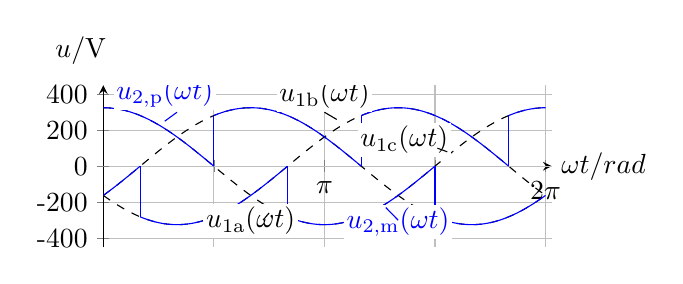
\begin{tikzpicture}
            \begin{axis}[
                % x/y range adjustment
                xmin=0, xmax=365,
                ymin=-450, ymax=450,
                samples=500,
                axis y line=center,
                axis x line=middle,
                extra y ticks=0,
                % Label text
                xlabel={$\omega t / \text{rad}$},,
                ylabel={$u/\mathrm{V}$},
                % Label adjustment
                x label style={at={(axis description cs:1,0.5)},anchor=west},
                y label style={at={(axis description cs:-.05,.97)},anchor=south,yshift=0.2cm},
                width=0.6\textwidth,
                height=0.3\textwidth,
                % x-Ticks
                xtick={0,90,180,270,360},
                xticklabels={,,$\pi$,,$2\pi$},
                xticklabel style = {anchor=north},
                % y-Ticks
                ytick={400,200,0,-200,-400},
                yticklabels={400,200,0,-200,-400},
                yticklabel style = {anchor=east},
                % Grid layout
                grid,
                %grid style={line width=.1pt, draw=gray!10},
                %major grid style={line width=.2pt,draw=gray!90},
            ]
            % Voltage u1a(wt), u1b(wt) u1c(wt)
            \addplot[black, domain= 0:360,dashed] {325*cos(x)};                
            \addplot[black, domain= 0:360,dashed] {325*cos(x+120)};                
            \addplot[black, domain= 0:360,dashed] {325*cos(x+240)}; 
            % Voltage u2p(wt)
            \addplot[blue, domain= 0:90] {325*cos(x)};                
            \addplot[blue, domain= 90:210] {325*cos(x+240)};                
            \addplot[blue, domain= 210:330] {325*cos(x+120)};
            \addplot[blue, domain= 330:360] {325*cos(x)};                
            \addplot[color=blue,solid] coordinates{
                (90,0)
                (90, 281.4)
            };     
            \addplot[color=blue,solid] coordinates{
                (210,0)
                (210, 281.4)
            };     
            \addplot[color=blue,solid] coordinates{
                (330,0)
                (330, 281.4)
            };     
         
            % Voltage u2m(wt)
            \addplot[blue, domain= 0:30] {325*cos(x+240)};                
            \addplot[blue, domain= 30:150] {325*cos(x+120)};                
            \addplot[blue, domain= 150:270] {325*cos(x)};                
            \addplot[blue, domain= 270:360] {325*cos(x+240)};
            \addplot[color=blue,solid] coordinates{
                (30,0)
                (30, -281.4)
            };     
            \addplot[color=blue,solid] coordinates{
                (150,0)
                (150, -281.4)
            };     
            \addplot[color=blue,solid] coordinates{
                (270,0)
                (270, -281.4)
            };     
        
            % Label of u1c
            \node[black, fill=white, inner sep = 1pt, anchor = south] at (axis cs:245,50) {$u_{\mathrm{1c}}(\omega t)$};
            % Line to u1a
            \draw[thin, black] (272,100) -- (280,80); 
            % Label of u1a
            \node[black, fill=white, inner sep = 1pt, anchor = south] at (axis cs:120,-400) {$u_{\mathrm{1a}}(\omega t)$};
            % Line to u1a
            \draw[thin, black] (130,-300) -- (135,-260);            
            % Label of u1b
            \node[black, fill=white, inner sep = 1pt, anchor = south] at (axis cs:180,300) {$u_{\mathrm{1b}}(\omega t)$};
            % Line to u1b
            \draw[thin, black] (180,300) -- (190,260);
            % Label of u2,p
            \node[blue, fill=white, inner sep = 1pt, anchor = south] at (axis cs:50,310) {$u_{\mathrm{2,p}}(\omega t)$};
            % Line to u2,p
            \draw[thin, blue] (60,300) -- (50,250);
            % Label of u2,m
            \node[blue, fill=white, inner sep = 1pt, anchor = south] at (axis cs:240,-410) {$u_{\mathrm{2,m}}(\omega t)$};
            % Line to u2,m
            \draw[thin, blue] (240,-300) -- (230,-230);
        \end{axis}     
        \end{tikzpicture}
        \caption{Output voltage $u_\mathrm{2,p}(t)$ and $u_\mathrm{2,m}(t)$ for raising load.}
        \label{sfig:ex06_Voltage_u2pmn_Raise}
\end{solutionfigure}

    In \autoref{sfig:ex06_Voltage_u2pm_Down} the output voltages are $\overline{u}_\mathrm{2,p}=\SI{-233}{\volt}$ and $\overline{u}_\mathrm{2,m}=\SI{233}{\volt}$.
    Also here the conducting state of the thyristors are entered.
    
    \input{fig/ex06/sFig_VoltageU2pmDown}

    

    \FloatBarrier

    In \autoref{sfig:ex06_Voltage_u2up_down} the output voltages are $\overline{u}_\mathrm{2}$ are entered for both cases.

    %%%%%%%%%%%%%%%%%%%%%%%%%%%%%%%%%%%%%%%%%%%%%%%%%%%%%%%%%%%%%%%%%%%%%%%%%%
% Signal of u2 for raising and lowing load
%%%%%%%%%%%%%%%%%%%%%%%%%%%%%%%%%%%%%%%%%%%%%%%%%%%%%%%%%%%%%%%%%%%%%%%%%%
\begin{solutionfigure}[htb]

 %   \documentclass{standalone}
 %   \usepackage{pgfplots}
 %   \pgfplotsset{compat=1.18} % Kompatibilität für neuere Versionen
        \centering
        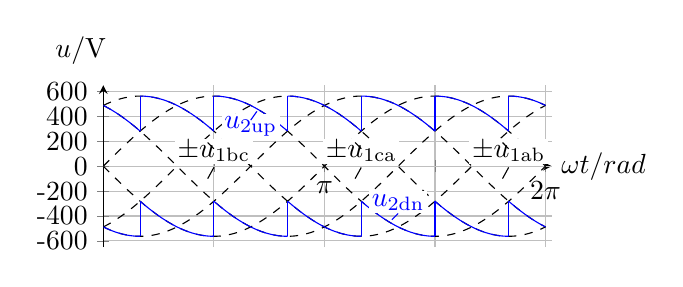
\begin{tikzpicture}
            \begin{axis}[
                % x/y range adjustment
                xmin=0, xmax=365,
                ymin=-650, ymax=650,
                samples=500,
                axis y line=center,
                axis x line=middle,
                extra y ticks=0,
                % Label text
                xlabel={$\omega t / \text{rad}$},,
                ylabel={$u/\mathrm{V}$},
                % Label adjustment
                x label style={at={(axis description cs:1,0.5)},anchor=west},
                y label style={at={(axis description cs:-.05,.97)},anchor=south,yshift=0.2cm},
                width=0.6\textwidth,
                height=0.3\textwidth,
                % x-Ticks
                xtick={0,90,180,270,360},
                xticklabels={,,$\pi$,,$2\pi$},
                xticklabel style = {anchor=north},
                % y-Ticks
                ytick={600,400,200,0,-200,-400,-600},
                yticklabels={600,400,200,0,-200,-400,-600},
                yticklabel style = {anchor=east},
                % Grid layout
                grid,
                %grid style={line width=.1pt, draw=gray!10},
                %major grid style={line width=.2pt,draw=gray!90},
            ]
            % Voltage u1ab(wt), u1bc(wt) u1ca(wt)
            \addplot[black, domain= 0:360,dashed] {563*cos(x-30)};                
            \addplot[black, domain= 0:360,dashed] {563*cos(x+90)};                
            \addplot[black, domain= 0:360,dashed] {563*cos(x+210)}; 
            % Voltage -u1ab(wt), -u1bc(wt) -u1ca(wt)
            \addplot[black, domain= 0:360,dashed] {-563*cos(x-30)};                
            \addplot[black, domain= 0:360,dashed] {-563*cos(x+90)};                
            \addplot[black, domain= 0:360,dashed] {-563*cos(x+210)}; 
            % Voltage u2(wt) up
            \addplot[blue, domain= 0:30] {-563*cos(x+210)};            
            \addplot[blue, domain= 30:90] {563*cos(x-30)};                
            \addplot[blue, domain= 270:330] {563*cos(x+90)};                
            \addplot[blue, domain= 150:210] {563*cos(x+210)}; 
            \addplot[blue, domain= 210:270] {-563*cos(x-30)};                
            \addplot[blue, domain= 90:150] {-563*cos(x+90)};                
            \addplot[blue, domain= 330:360] {-563*cos(x+210)};            
            \addplot[color=blue,solid] coordinates{
                (30, 563)
                (30, 282)
            };     
            \addplot[color=blue,solid] coordinates{
                (90, 563)
                (90, 282)
            };     
            \addplot[color=blue,solid] coordinates{
                (150, 563)
                (150, 282)
            };     
            \addplot[color=blue,solid] coordinates{
                (210, 563)
                (210, 282)
            };     
            \addplot[color=blue,solid] coordinates{
                (270, 563)
                (270, 282)
            };     
            \addplot[color=blue,solid] coordinates{
                (330, 563)
                (330, 282)
            };     
    
            % Voltage u2(wt) down
            \addplot[blue, domain= 0:30] {-563*cos(x-30)};                
            \addplot[blue, domain= 150:210] {563*cos(x-30)};                
            \addplot[blue, domain= 30:90] {563*cos(x+90)};                
            \addplot[blue, domain= 270:330] {563*cos(x+210)};            
            \addplot[blue, domain= 330:360] {-563*cos(x-30)};                
            \addplot[blue, domain= 210:270] {-563*cos(x+90)};                
            \addplot[blue, domain= 90:150] {-563*cos(x+210)}; 
            \addplot[color=blue,solid] coordinates{
                (30,-563)
                (30,-282)
            };     
            \addplot[color=blue,solid] coordinates{
                (90,-563)
                (90,-282)
            };     
            \addplot[color=blue,solid] coordinates{
                (150,-563)
                (150,-282)
            };     
            \addplot[color=blue,solid] coordinates{
                (210,-563)
                (210,-282)
            };     
            \addplot[color=blue,solid] coordinates{
                (270,-563)
                (270,-282)
            };     
            \addplot[color=blue,solid] coordinates{
                (330,-563)
                (330,-282)
            };     
         
            % Label of +-u1bc
            \node[black, fill=white, inner sep = 1pt, anchor = south] at (axis cs:90,10) {$\pm u_{\mathrm{1bc}}$};
            % Line to +u1bc
            \draw[thin, black] (90,140) -- (85,190);            
            % Line to -u1bc
            \draw[thin, black] (90,-10) -- (85,-100);            
            % Label of +-u1ca
            \node[black, fill=white, inner sep = 1pt, anchor = south] at (axis cs:210,10) {$\pm u_{\mathrm{1ca}}$};
            % Line to +u1ca
            \draw[thin, black] (210,140) -- (205,190);            
            % Line to -u1ca
            \draw[thin, black] (210,-10) -- (205,-100);   
            % Label of +-u1ab
            \node[black, fill=white, inner sep = 1pt, anchor = south] at (axis cs:330,10) {$\pm u_{\mathrm{1ab}}$};
            % Line to +u1ab
            \draw[thin, black] (330,140) -- (325,190);            
            % Line to -u1ab
            \draw[thin, black] (330,-10) -- (325,-100);               
            % Label of u2up
            \node[blue, fill=white, inner sep = 1pt, anchor = south] at (axis cs:120,210) {$u_{\mathrm{2 up}}$};
            % Line to u2,p
            \draw[thin, blue] (120,370) -- (125,440);
            % Label of u2,m
            \node[blue, fill=white, inner sep = 1pt, anchor = south] at (axis cs:240,-380) {$u_{\mathrm{2 dn}}$};
            % Line to u2,m
            \draw[thin, blue] (240,-380) -- (235,-430);
        \end{axis}     
        \end{tikzpicture}
        \caption{Output voltage $u_\mathrm{2 up}(\omega t)$ for raising and $u_\mathrm{2 dn}(\omega t)$ lowing load.}
        \label{sfig:ex06_Voltage_u2pmn_down}
\end{solutionfigure}

    \FloatBarrier

    The amplitude of the fundamental $i_\mathrm{1a}^\mathrm{(1)}(t)$ is determined by calculating the Fourier coefficient.
    To simplify the calculation the the current signal $i_\mathrm{1a}(t)$ is shift $\frac{2 \pi}{3}\SI{}{\radian}$ to the left, 
    so that it is axially symmetric. Cause by the symmetry the integration is performed only from \SI{0}{\radian} to \SI{\pi}{\radian}:
    \begin{equation}
        \begin{split}
            \hat{i}_\mathrm{1a}^\mathrm{(1)} &= \frac{2}{\pi} \int_{0}^{\pi} i_\mathrm{1a}(\omega t) \cos(\omega t) \mathrm{d}\omega t=
            \frac{2}{\pi} \left( \int_{0}^{\frac{\pi}{3}} I\mathrm{mot} \cos(\omega t) \mathrm{d}\omega t 
            - \int_{\frac{2\pi}{3}}^{\pi} I_\mathrm{mot} \cos(\omega t) \mathrm{d}\omega t \right)  \\
            &= \frac{2 I_\mathrm{mot}}{\pi} \left( \sin(\frac{\pi}{3}) + \sin(\frac{2\pi}{3}) \right) 
            = \frac{2\cdot \SI{20}{\ampere}}{\pi} \sqrt{3}= \SI{22}{\ampere}.
        \end{split}
    \end{equation}
    The result is valid for raising and lowering load, because in both cases the rectangle width and relative positions are the same.
    The difference belongs only to the phase position relative to $U_\mathrm{1}(t)$.

    \input{fig/ex06/sFig_CurrentI1up}

    \input{fig/ex06/sFig_CurrentI1down}
    
    \FloatBarrier

    The voltage $u_\mathrm{T1}(t)$ is displayed for raising load in \autoref{sfig:ex06_Voltage_u1T_up}  and for lowering load in \autoref{sfig:ex06_Voltage_u1T_down}.

    \input{fig/ex06/sFig_VoltageUT1Up}

    \input{fig/ex06/sFig_VoltageUT1Down}
    
\end{solutionblock}

% Subtask3
\subtask{Calculate the active power $P$, the fundamental reactive power $Q^\mathrm{(1)}$
and the fundamental apparent power $S^\mathrm{(1)}$ for the two considered operating points. Represent $P$, $Q^\mathrm{(1)}$ and $S^\mathrm{(1)}$ in the complex plane.}
\begin{solutionblock}
    \begin{equation}
        \begin{split}
            P_\mathrm{up}&=U_\mathrm{mot} I_\mathrm{mot}=\SI{466}{\volt} \cdot \SI{20}{\ampere}= \SI{9320}{\watt}. \\
            P_\mathrm{down}&=-U_\mathrm{mot} I_\mathrm{mot}=\SI{-466}{\volt} \cdot \SI{20}{\ampere}= \SI{9320}{\watt}.
        \end{split}
    \end{equation}
    The input voltage $U_\mathrm{1}^\mathrm{(1)}$ corresponds to $U_\mathrm{1}$, so that the apparent power results to
    \begin{equation}
        \begin{split}
            S_\mathrm{up}^\mathrm{(1)}&=3 U_\mathrm{1} \frac{\hat{i}_\mathrm{1a}^\mathrm{(1)}}{\sqrt{2}}=\SI{230}{\volt} \cdot \frac{\SI{22}{\ampere}}{\sqrt{2}}= \SI{10760}{\watt}. \\
            S_\mathrm{down}^\mathrm{(1)}&=3 U_\mathrm{1} \frac{\hat{i}_\mathrm{1a}^\mathrm{(1)}}{\sqrt{2}}=\SI{230}{\volt} \cdot \frac{\SI{22}{\ampere}}{\sqrt{2}}= \SI{10760}{\watt}.
        \end{split}
    \end{equation}
    The reactive power is calculated by
    \begin{equation}
        \begin{split}
            Q_\mathrm{up}^\mathrm{(1)}&=3 U_\mathrm{1} \frac{\hat{i}_\mathrm{1a}^\mathrm{(1)}}{\sqrt{2}} \sin{(\alpha_\mathrm{up})}
            =\SI{230}{\volt} \cdot \frac{\SI{22}{\ampere}}{\sqrt{2}}\sin{(\frac{\pi}{6})}= \SI{5380}{\watt}. \\
            Q_\mathrm{down}^\mathrm{(1)}&=3 U_\mathrm{1} \frac{-\hat{i}_\mathrm{1a}^\mathrm{(1)}}{\sqrt{2}} \sin{(\alpha_\mathrm{down})}
            =\SI{230}{\volt} \cdot \frac{\SI{22}{\ampere}}{\sqrt{2}}\sin{(\frac{5\pi}{6})}= \SI{5380}{\watt}.
        \end{split}
    \end{equation}
    \autoref{fig:ex06_Complex_Plane_Power} shows the power in the complex plane.

    %%%%%%%%%%%%%%%%%%%%%%%%%%%%%%%%%%%%%%%%%%%%%%%%%%%%%%%%%%%%%%%%%%%%%%%%%%
% Signal of uT1 for raising load
%%%%%%%%%%%%%%%%%%%%%%%%%%%%%%%%%%%%%%%%%%%%%%%%%%%%%%%%%%%%%%%%%%%%%%%%%%
\begin{solutionfigure}[htb]

 %   \documentclass{standalone}
 %   \usepackage{pgfplots}
 %   \pgfplotsset{compat=1.18} % Kompatibilität für neuere Versionen
        \centering
        \begin{tikzpicture}
            \tikzmath{
                real \ac, \i2, \ic;
                \i2 = 1; % load current
                \ic = 9; % commutation current
                \ac = 180 - acos(\i2/\ic -1); % firing angle margin for commutation
            }
            \begin{axis}[
                % x/y range adjustment
                xmin=-6200, xmax=6200,
                ymin=-1000, ymax=12300,
                samples=500,
                axis y line=center,
                axis x line=middle,
                extra y ticks=0,
                % Label text
                xlabel={$active power/ \SI{}{\kilo\watt}$},,
                ylabel={$reactive power/ \SI{}{\kilo\watt}$},
                % Label adjustment
                x label style={at={(axis description cs:1,0.5)},anchor=west},
                y label style={at={(axis description cs:-.05,.97)},anchor=south,yshift=0.2cm},
                width=0.6\textwidth,
                height=0.3\textwidth,
                % x-Ticks
                xtick={6000,4000,2000,0,-2000,-4000,-6000},
                xticklabels={6,4,2,0,-2,-4,-6},
                xticklabel style = {anchor=north},
                % y-Ticks
                ytick={0,3000,6000,9000,12000},
                yticklabels={,3,6,9,12},
                yticklabel style = {anchor=east},
                % Grid layout
                grid,
                %grid style={line width=.1pt, draw=gray!10},
                %major grid style={line width=.2pt,draw=gray!90},
                ]
            \end{axis}
        \end{tikzpicture}
        \caption{Power within the complex plane}
        \label{fig:ex06_Complex_Plane_Power}

\end{solutionfigure}

\end{solutionblock}
% Subtask4
\subtask{Calculate the fundamental current ratio $g=\frac{I^\mathrm{(1)}}{I}$ and the power factor $\lambda$ for the two considered operating points.}
\begin{solutionblock}
    The fundamental current ratio results to
    \begin{equation}
        g=\frac{\frac{\hat{i}_\mathrm{1a}^\mathrm{(1)}}{\sqrt{2}}}{I_\mathrm{mot}}=\frac{\frac{\SI{22}{\ampere}}{\sqrt{2}}}{\SI{20}{\ampere}}=0.78.
    \end{equation}
    The power factor $\lambda$ is calculated by
    \begin{equation}
        \begin{split}
            \lambda_\mathrm{up}&=g \cdot \cos{(\alpha_\mathrm{up})}=0.78  \cdot cos(\frac{\pi}{6})= 0.68. \\
            \lambda_\mathrm{down}&=g \cdot \cos{(\alpha_\mathrm{down})}=0.78  \cdot cos(\frac{5\pi}{6})= -0.68.
        \end{split}
    \end{equation}
\end{solutionblock}
